\documentclass[1p]{elsarticle_modified}
%\bibliographystyle{elsarticle-num}

%\usepackage[colorlinks]{hyperref}
%\usepackage{abbrmath_seonhwa} %\Abb, \Ascr, \Acal ,\Abf, \Afrak
\usepackage{amsfonts}
\usepackage{amssymb}
\usepackage{amsmath}
\usepackage{amsthm}
\usepackage{scalefnt}
\usepackage{amsbsy}
\usepackage{kotex}
\usepackage{caption}
\usepackage{subfig}
\usepackage{color}
\usepackage{graphicx}
\usepackage{xcolor} %% white, black, red, green, blue, cyan, magenta, yellow
\usepackage{float}
\usepackage{setspace}
\usepackage{hyperref}

\usepackage{tikz}
\usetikzlibrary{arrows}

\usepackage{multirow}
\usepackage{array} % fixed length table
\usepackage{hhline}

%%%%%%%%%%%%%%%%%%%%%
\makeatletter
\renewcommand*\env@matrix[1][\arraystretch]{%
	\edef\arraystretch{#1}%
	\hskip -\arraycolsep
	\let\@ifnextchar\new@ifnextchar
	\array{*\c@MaxMatrixCols c}}
\makeatother %https://tex.stackexchange.com/questions/14071/how-can-i-increase-the-line-spacing-in-a-matrix
%%%%%%%%%%%%%%%

\usepackage[normalem]{ulem}

\newcommand{\msout}[1]{\ifmmode\text{\sout{\ensuremath{#1}}}\else\sout{#1}\fi}
%SOURCE: \msout is \stkout macro in https://tex.stackexchange.com/questions/20609/strikeout-in-math-mode

\newcommand{\cancel}[1]{
	\ifmmode
	{\color{red}\msout{#1}}
	\else
	{\color{red}\sout{#1}}
	\fi
}

\newcommand{\add}[1]{
	{\color{blue}\uwave{#1}}
}

\newcommand{\replace}[2]{
	\ifmmode
	{\color{red}\msout{#1}}{\color{blue}\uwave{#2}}
	\else
	{\color{red}\sout{#1}}{\color{blue}\uwave{#2}}
	\fi
}

\newcommand{\Sol}{\mathcal{S}} %segment
\newcommand{\D}{D} %diagram
\newcommand{\A}{\mathcal{A}} %arc


%%%%%%%%%%%%%%%%%%%%%%%%%%%%%5 test

\def\sl{\operatorname{\textup{SL}}(2,\Cbb)}
\def\psl{\operatorname{\textup{PSL}}(2,\Cbb)}
\def\quan{\mkern 1mu \triangleright \mkern 1mu}

\theoremstyle{definition}
\newtheorem{thm}{Theorem}[section]
\newtheorem{prop}[thm]{Proposition}
\newtheorem{lem}[thm]{Lemma}
\newtheorem{ques}[thm]{Question}
\newtheorem{cor}[thm]{Corollary}
\newtheorem{defn}[thm]{Definition}
\newtheorem{exam}[thm]{Example}
\newtheorem{rmk}[thm]{Remark}
\newtheorem{alg}[thm]{Algorithm}

\newcommand{\I}{\sqrt{-1}}
\begin{document}

%\begin{frontmatter}
%
%\title{Boundary parabolic representations of knots up to 8 crossings}
%
%%% Group authors per affiliation:
%\author{Yunhi Cho} 
%\address{Department of Mathematics, University of Seoul, Seoul, Korea}
%\ead{yhcho@uos.ac.kr}
%
%
%\author{Seonhwa Kim} %\fnref{s_kim}}
%\address{Center for Geometry and Physics, Institute for Basic Science, Pohang, 37673, Korea}
%\ead{ryeona17@ibs.re.kr}
%
%\author{Hyuk Kim}
%\address{Department of Mathematical Sciences, Seoul National University, Seoul 08826, Korea}
%\ead{hyukkim@snu.ac.kr}
%
%\author{Seokbeom Yoon}
%\address{Department of Mathematical Sciences, Seoul National University, Seoul, 08826,  Korea}
%\ead{sbyoon15@snu.ac.kr}
%
%\begin{abstract}
%We find all boundary parabolic representation of knots up to 8 crossings.
%
%\end{abstract}
%\begin{keyword}
%    \MSC[2010] 57M25 
%\end{keyword}
%
%\end{frontmatter}

%\linenumbers
%\tableofcontents
%
\newcommand\colored[1]{\textcolor{white}{\rule[-0.35ex]{0.8em}{1.4ex}}\kern-0.8em\color{red} #1}%
%\newcommand\colored[1]{\textcolor{white}{ #1}\kern-2.17ex	\textcolor{white}{ #1}\kern-1.81ex	\textcolor{white}{ #1}\kern-2.15ex\color{red}#1	}

{\Large $\underline{10_{79}~(K10a_{78})}$}

\setlength{\tabcolsep}{10pt}
\renewcommand{\arraystretch}{1.6}
\vspace{1cm}\begin{tabular}{m{100pt}>{\centering\arraybackslash}m{274pt}}
\multirow{5}{120pt}{
	\centering
	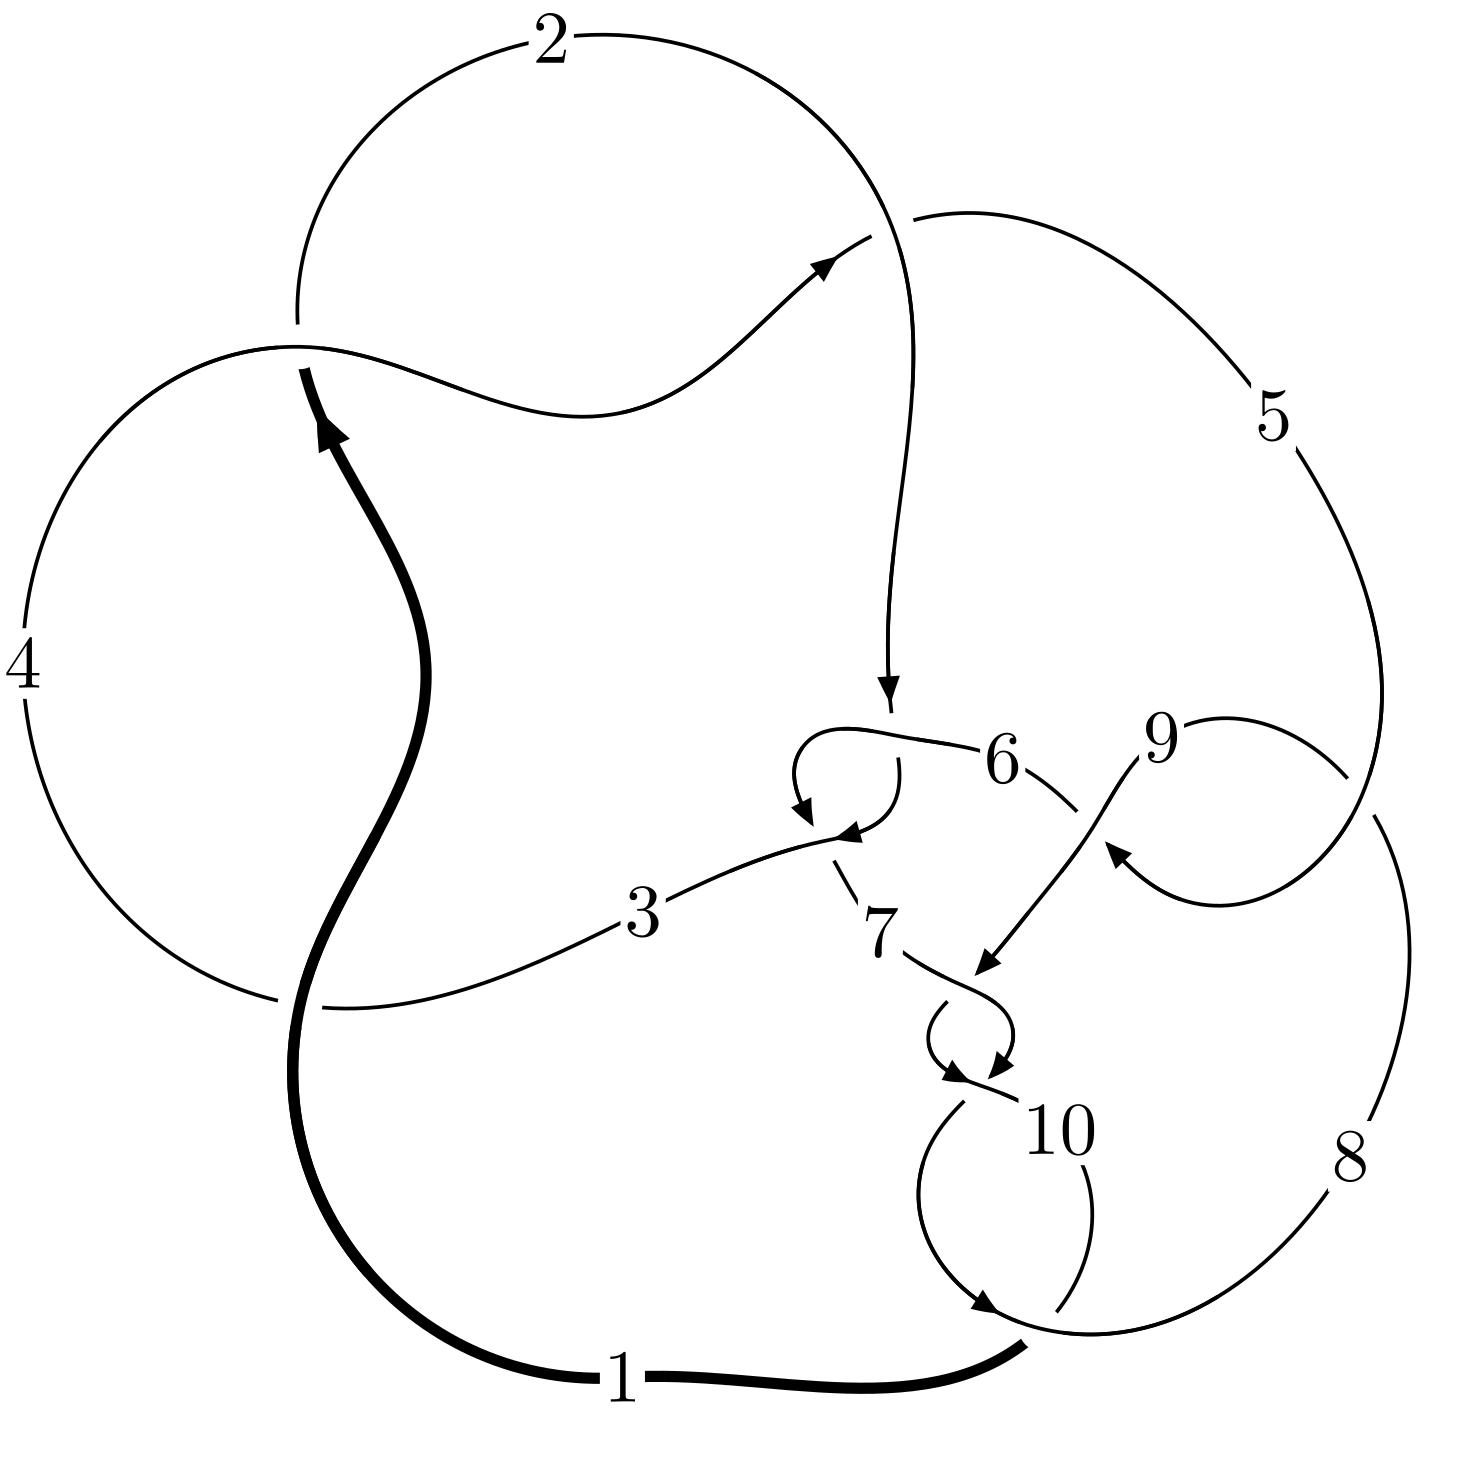
\includegraphics[width=112pt]{../../../GIT/diagram.site/Diagrams/png/163_10_79.png}\\
\ \ \ A knot diagram\footnotemark}&
\allowdisplaybreaks
\textbf{Linearized knot diagam} \\
\cline{2-2}
 &
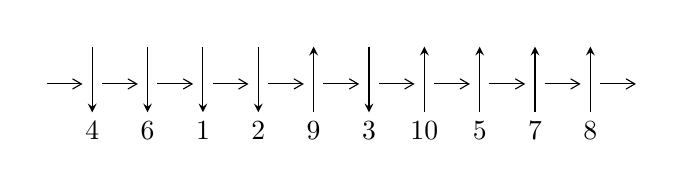
\begin{tikzpicture}[x=20pt, y=17pt]
	% nodes
	\node (C0) at (0, 0) {};
	\node (C1) at (1, 0) {};
	\node (C1U) at (1, +1) {};
	\node (C1D) at (1, -1) {4};

	\node (C2) at (2, 0) {};
	\node (C2U) at (2, +1) {};
	\node (C2D) at (2, -1) {6};

	\node (C3) at (3, 0) {};
	\node (C3U) at (3, +1) {};
	\node (C3D) at (3, -1) {1};

	\node (C4) at (4, 0) {};
	\node (C4U) at (4, +1) {};
	\node (C4D) at (4, -1) {2};

	\node (C5) at (5, 0) {};
	\node (C5U) at (5, +1) {};
	\node (C5D) at (5, -1) {9};

	\node (C6) at (6, 0) {};
	\node (C6U) at (6, +1) {};
	\node (C6D) at (6, -1) {3};

	\node (C7) at (7, 0) {};
	\node (C7U) at (7, +1) {};
	\node (C7D) at (7, -1) {10};

	\node (C8) at (8, 0) {};
	\node (C8U) at (8, +1) {};
	\node (C8D) at (8, -1) {5};

	\node (C9) at (9, 0) {};
	\node (C9U) at (9, +1) {};
	\node (C9D) at (9, -1) {7};

	\node (C10) at (10, 0) {};
	\node (C10U) at (10, +1) {};
	\node (C10D) at (10, -1) {8};
	\node (C11) at (11, 0) {};

	% arrows
	\draw[->,>={angle 60}]
	(C0) edge (C1) (C1) edge (C2) (C2) edge (C3) (C3) edge (C4) (C4) edge (C5) (C5) edge (C6) (C6) edge (C7) (C7) edge (C8) (C8) edge (C9) (C9) edge (C10) (C10) edge (C11) ;	\draw[->,>=stealth]
	(C1U) edge (C1D) (C2U) edge (C2D) (C3U) edge (C3D) (C4U) edge (C4D) (C5D) edge (C5U) (C6U) edge (C6D) (C7D) edge (C7U) (C8D) edge (C8U) (C9D) edge (C9U) (C10D) edge (C10U) ;
	\end{tikzpicture} \\
\hhline{~~} \\& 
\textbf{Solving Sequence} \\ \cline{2-2} 
 &
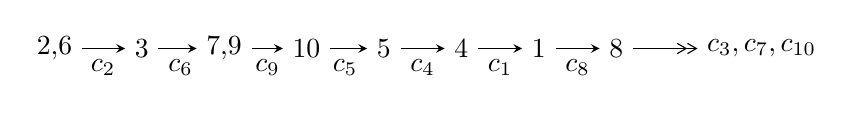
\begin{tikzpicture}[x=28pt, y=7pt]
	% node
	\node (A0) at (-1/8, 0) {2,6};
	\node (A1) at (1, 0) {3};
	\node (A2) at (33/16, 0) {7,9};
	\node (A3) at (25/8, 0) {10};
	\node (A4) at (33/8, 0) {5};
	\node (A5) at (41/8, 0) {4};
	\node (A6) at (49/8, 0) {1};
	\node (A7) at (57/8, 0) {8};
	\node (C1) at (1/2, -1) {$c_{2}$};
	\node (C2) at (3/2, -1) {$c_{6}$};
	\node (C3) at (21/8, -1) {$c_{9}$};
	\node (C4) at (29/8, -1) {$c_{5}$};
	\node (C5) at (37/8, -1) {$c_{4}$};
	\node (C6) at (45/8, -1) {$c_{1}$};
	\node (C7) at (53/8, -1) {$c_{8}$};
	\node (A8) at (9, 0) {$c_{3},c_{7},c_{10}$};

	% edge
	\draw[->,>=stealth]	
	(A0) edge (A1) (A1) edge (A2) (A2) edge (A3) (A3) edge (A4) (A4) edge (A5) (A5) edge (A6) (A6) edge (A7) ;
	\draw[->>,>={angle 60}]	
	(A7) edge (A8);
\end{tikzpicture} \\ 

\end{tabular} \\

\footnotetext{
The image of knot diagram is generated by the software ``\textbf{Draw programme}" developed by Andrew Bartholomew(\url{http://www.layer8.co.uk/maths/draw/index.htm\#Running-draw}), where we modified some parts for our purpose(\url{https://github.com/CATsTAILs/LinksPainter}).
}\phantom \\ \newline 
\centering \textbf{Ideals for irreducible components\footnotemark of $X_{\text{par}}$} 
 
\begin{align*}
I^u_{1}&=\langle 
1.48752\times10^{31} u^{33}-1.92107\times10^{31} u^{32}+\cdots+2.67160\times10^{30} b-8.42537\times10^{31},\\
\phantom{I^u_{1}}&\phantom{= \langle  }2.31853\times10^{30} u^{33}-3.45308\times10^{30} u^{32}+\cdots+7.63313\times10^{29} a-1.53986\times10^{31},\;u^{34}-2 u^{33}+\cdots-4 u+4\rangle \\
I^u_{2}&=\langle 
b- u-1,\;a,\;u^2+u-1\rangle \\
\\
I^v_{1}&=\langle 
a,\;b- v+2,\;v^2-3 v+1\rangle \\
\end{align*}
\raggedright * 3 irreducible components of $\dim_{\mathbb{C}}=0$, with total 38 representations.\\
\footnotetext{All coefficients of polynomials are rational numbers. But the coefficients are sometimes approximated in decimal forms when there is not enough margin.}
\newpage
\renewcommand{\arraystretch}{1}
\centering \section*{I. $I^u_{1}= \langle 1.49\times10^{31} u^{33}-1.92\times10^{31} u^{32}+\cdots+2.67\times10^{30} b-8.43\times10^{31},\;2.32\times10^{30} u^{33}-3.45\times10^{30} u^{32}+\cdots+7.63\times10^{29} a-1.54\times10^{31},\;u^{34}-2 u^{33}+\cdots-4 u+4 \rangle$}
\flushleft \textbf{(i) Arc colorings}\\
\begin{tabular}{m{7pt} m{180pt} m{7pt} m{180pt} }
\flushright $a_{2}=$&$\begin{pmatrix}1\\0\end{pmatrix}$ \\
\flushright $a_{6}=$&$\begin{pmatrix}0\\u\end{pmatrix}$ \\
\flushright $a_{3}=$&$\begin{pmatrix}1\\u^2\end{pmatrix}$ \\
\flushright $a_{7}=$&$\begin{pmatrix}- u\\- u^3+u\end{pmatrix}$ \\
\flushright $a_{9}=$&$\begin{pmatrix}-3.03746 u^{33}+4.52380 u^{32}+\cdots+15.5234 u+20.1734\\-5.56789 u^{33}+7.19074 u^{32}+\cdots+16.8842 u+31.5368\end{pmatrix}$ \\
\flushright $a_{10}=$&$\begin{pmatrix}-6.74042 u^{33}+9.34081 u^{32}+\cdots+25.8322 u+41.5551\\-3.71677 u^{33}+4.73023 u^{32}+\cdots+11.0317 u+20.5108\end{pmatrix}$ \\
\flushright $a_{5}=$&$\begin{pmatrix}-8.87471 u^{33}+12.3007 u^{32}+\cdots+32.0519 u+57.5877\\-5.70723 u^{33}+7.43204 u^{32}+\cdots+16.7561 u+33.4853\end{pmatrix}$ \\
\flushright $a_{4}=$&$\begin{pmatrix}-14.5819 u^{33}+19.7327 u^{32}+\cdots+48.8081 u+91.0730\\-5.70723 u^{33}+7.43204 u^{32}+\cdots+16.7561 u+33.4853\end{pmatrix}$ \\
\flushright $a_{1}=$&$\begin{pmatrix}-14.5819 u^{33}+19.7327 u^{32}+\cdots+48.8081 u+91.0730\\-0.387583 u^{33}+0.811626 u^{32}+\cdots+3.84702 u+4.23934\end{pmatrix}$ \\
\flushright $a_{8}=$&$\begin{pmatrix}15.6894 u^{33}-20.9276 u^{32}+\cdots-48.8834 u-95.7780\\1.33189 u^{33}-1.83094 u^{32}+\cdots-2.59403 u-8.86592\end{pmatrix}$\\&\end{tabular}
\flushleft \textbf{(ii) Obstruction class $= -1$}\\~\\
\flushleft \textbf{(iii) Cusp Shapes $= 3.23572 u^{33}-4.86218 u^{32}+\cdots-45.6005 u-20.0908$}\\~\\
\newpage\renewcommand{\arraystretch}{1}
\flushleft \textbf{(iv) u-Polynomials at the component}\newline \\
\begin{tabular}{m{50pt}|m{274pt}}
Crossings & \hspace{64pt}u-Polynomials at each crossing \\
\hline $$\begin{aligned}c_{1},c_{3},c_{4}\end{aligned}$$&$\begin{aligned}
&u^{34}-4 u^{33}+\cdots+10 u+1
\end{aligned}$\\
\hline $$\begin{aligned}c_{2},c_{6}\end{aligned}$$&$\begin{aligned}
&u^{34}+2 u^{33}+\cdots+4 u+4
\end{aligned}$\\
\hline $$\begin{aligned}c_{5},c_{8}\end{aligned}$$&$\begin{aligned}
&u^{34}-2 u^{33}+\cdots-4 u+4
\end{aligned}$\\
\hline $$\begin{aligned}c_{7},c_{9},c_{10}\end{aligned}$$&$\begin{aligned}
&u^{34}+4 u^{33}+\cdots-10 u+1
\end{aligned}$\\
\hline
\end{tabular}\\~\\
\newpage\renewcommand{\arraystretch}{1}
\flushleft \textbf{(v) Riley Polynomials at the component}\newline \\
\begin{tabular}{m{50pt}|m{274pt}}
Crossings & \hspace{64pt}Riley Polynomials at each crossing \\
\hline $$\begin{aligned}c_{1},c_{3},c_{4}\\c_{7},c_{9},c_{10}\end{aligned}$$&$\begin{aligned}
&y^{34}-32 y^{33}+\cdots-42 y+1
\end{aligned}$\\
\hline $$\begin{aligned}c_{2},c_{5},c_{6}\\c_{8}\end{aligned}$$&$\begin{aligned}
&y^{34}-18 y^{33}+\cdots-296 y+16
\end{aligned}$\\
\hline
\end{tabular}\\~\\
\newpage\flushleft \textbf{(vi) Complex Volumes and Cusp Shapes}
$$\begin{array}{c|c|c}  
\text{Solutions to }I^u_{1}& \I (\text{vol} + \sqrt{-1}CS) & \text{Cusp shape}\\
 \hline 
\begin{aligned}
u &= -0.334121 + 0.939075 I \\
a &= \phantom{-}0.665187 + 1.185390 I \\
b &= \phantom{-}0.168561 - 1.149830 I\end{aligned}
 & \phantom{-}8.19540 - 1.89242 I & \phantom{-}7.34522 + 1.79557 I \\ \hline\begin{aligned}
u &= -0.334121 - 0.939075 I \\
a &= \phantom{-}0.665187 - 1.185390 I \\
b &= \phantom{-}0.168561 + 1.149830 I\end{aligned}
 & \phantom{-}8.19540 + 1.89242 I & \phantom{-}7.34522 - 1.79557 I \\ \hline\begin{aligned}
u &= \phantom{-}0.286460 + 0.973864 I \\
a &= \phantom{-}0.697313 - 0.627321 I \\
b &= -0.30439 + 1.55545 I\end{aligned}
 & -2.64192 + 2.05432 I & -2.87162 - 3.29014 I \\ \hline\begin{aligned}
u &= \phantom{-}0.286460 - 0.973864 I \\
a &= \phantom{-}0.697313 + 0.627321 I \\
b &= -0.30439 - 1.55545 I\end{aligned}
 & -2.64192 - 2.05432 I & -2.87162 + 3.29014 I \\ \hline\begin{aligned}
u &= \phantom{-}0.810678 + 0.499386 I \\
a &= \phantom{-}0.792602 + 0.713045 I \\
b &= \phantom{-}0.050287 - 0.622907 I\end{aligned}
 & \phantom{-}2.64192 - 2.05432 I & \phantom{-}2.87162 + 3.29014 I \\ \hline\begin{aligned}
u &= \phantom{-}0.810678 - 0.499386 I \\
a &= \phantom{-}0.792602 - 0.713045 I \\
b &= \phantom{-}0.050287 + 0.622907 I\end{aligned}
 & \phantom{-}2.64192 + 2.05432 I & \phantom{-}2.87162 - 3.29014 I \\ \hline\begin{aligned}
u &= -0.995699 + 0.467507 I \\
a &= \phantom{-}0.638734 + 0.769428 I \\
b &= \phantom{-}0.60499 - 1.49342 I\end{aligned}
 & \phantom{-0.000000 -}4.00435 I & \phantom{-0.000000 } 0. - 6.49701 I \\ \hline\begin{aligned}
u &= -0.995699 - 0.467507 I \\
a &= \phantom{-}0.638734 - 0.769428 I \\
b &= \phantom{-}0.60499 + 1.49342 I\end{aligned}
 & \phantom{-0.000000 } -4.00435 I & \phantom{-0.000000 -}0. + 6.49701 I \\ \hline\begin{aligned}
u &= \phantom{-}1.088970 + 0.372927 I \\
a &= \phantom{-}0.911686 - 0.699013 I \\
b &= \phantom{-}1.62610 + 0.98618 I\end{aligned}
 & -3.39729 - 2.12414 I & -2.18234 + 2.03948 I \\ \hline\begin{aligned}
u &= \phantom{-}1.088970 - 0.372927 I \\
a &= \phantom{-}0.911686 + 0.699013 I \\
b &= \phantom{-}1.62610 - 0.98618 I\end{aligned}
 & -3.39729 + 2.12414 I & -2.18234 - 2.03948 I\\
 \hline 
 \end{array}$$\newpage$$\begin{array}{c|c|c}  
\text{Solutions to }I^u_{1}& \I (\text{vol} + \sqrt{-1}CS) & \text{Cusp shape}\\
 \hline 
\begin{aligned}
u &= \phantom{-}0.845756 + 0.036069 I \\
a &= -0.613787 + 0.538660 I \\
b &= \phantom{-}0.203218 - 0.673856 I\end{aligned}
 & -1.359860 + 0.095322 I & -5.80027 + 0.42636 I \\ \hline\begin{aligned}
u &= \phantom{-}0.845756 - 0.036069 I \\
a &= -0.613787 - 0.538660 I \\
b &= \phantom{-}0.203218 + 0.673856 I\end{aligned}
 & -1.359860 - 0.095322 I & -5.80027 - 0.42636 I \\ \hline\begin{aligned}
u &= -1.112820 + 0.516604 I \\
a &= -0.842410 + 0.743758 I \\
b &= -0.101206 + 0.252455 I\end{aligned}
 & -2.34523 + 5.26340 I & -1.79194 - 3.97493 I \\ \hline\begin{aligned}
u &= -1.112820 - 0.516604 I \\
a &= -0.842410 - 0.743758 I \\
b &= -0.101206 - 0.252455 I\end{aligned}
 & -2.34523 - 5.26340 I & -1.79194 + 3.97493 I \\ \hline\begin{aligned}
u &= -0.304859 + 0.635319 I \\
a &= -0.625675 + 0.780084 I \\
b &= \phantom{-}0.24828 - 2.17048 I\end{aligned}
 & \phantom{-0.000000 } -0.739532 I & \phantom{-0.000000 } 0. - 4.35806 I \\ \hline\begin{aligned}
u &= -0.304859 - 0.635319 I \\
a &= -0.625675 - 0.780084 I \\
b &= \phantom{-}0.24828 + 2.17048 I\end{aligned}
 & \phantom{-0.000000 -}0.739532 I & \phantom{-0.000000 -}0. + 4.35806 I \\ \hline\begin{aligned}
u &= -0.538543 + 0.433436 I \\
a &= -0.920373 - 0.807720 I \\
b &= -0.674327 + 1.021010 I\end{aligned}
 & \phantom{-}1.359860 - 0.095322 I & \phantom{-}5.80027 - 0.42636 I \\ \hline\begin{aligned}
u &= -0.538543 - 0.433436 I \\
a &= -0.920373 + 0.807720 I \\
b &= -0.674327 - 1.021010 I\end{aligned}
 & \phantom{-}1.359860 + 0.095322 I & \phantom{-}5.80027 + 0.42636 I \\ \hline\begin{aligned}
u &= \phantom{-}1.253480 + 0.421212 I \\
a &= \phantom{-}0.690781 - 0.529640 I \\
b &= -0.104017 + 0.977410 I\end{aligned}
 & \phantom{-}3.39729 - 2.12414 I & \phantom{-}2.18234 + 2.03948 I \\ \hline\begin{aligned}
u &= \phantom{-}1.253480 - 0.421212 I \\
a &= \phantom{-}0.690781 + 0.529640 I \\
b &= -0.104017 - 0.977410 I\end{aligned}
 & \phantom{-}3.39729 + 2.12414 I & \phantom{-}2.18234 - 2.03948 I\\
 \hline 
 \end{array}$$\newpage$$\begin{array}{c|c|c}  
\text{Solutions to }I^u_{1}& \I (\text{vol} + \sqrt{-1}CS) & \text{Cusp shape}\\
 \hline 
\begin{aligned}
u &= \phantom{-}0.650050\phantom{ +0.000000I} \\
a &= -2.72250\phantom{ +0.000000I} \\
b &= -1.02677\phantom{ +0.000000I}\end{aligned}
 & \phantom{-}6.73970\phantom{ +0.000000I} & -7.32000\phantom{ +0.000000I} \\ \hline\begin{aligned}
u &= -1.335420 + 0.228599 I \\
a &= \phantom{-}0.360026 - 0.641577 I \\
b &= \phantom{-}0.062959 - 0.180613 I\end{aligned}
 & -8.19540 + 1.89242 I & -7.34522 - 1.79557 I \\ \hline\begin{aligned}
u &= -1.335420 - 0.228599 I \\
a &= \phantom{-}0.360026 + 0.641577 I \\
b &= \phantom{-}0.062959 + 0.180613 I\end{aligned}
 & -8.19540 - 1.89242 I & -7.34522 + 1.79557 I \\ \hline\begin{aligned}
u &= \phantom{-}1.215470 + 0.599118 I \\
a &= -0.588471 + 0.824257 I \\
b &= -1.38976 - 1.48159 I\end{aligned}
 & -5.53452 - 7.73594 I & -3.53535 + 5.97450 I \\ \hline\begin{aligned}
u &= \phantom{-}1.215470 - 0.599118 I \\
a &= -0.588471 - 0.824257 I \\
b &= -1.38976 + 1.48159 I\end{aligned}
 & -5.53452 + 7.73594 I & -3.53535 - 5.97450 I \\ \hline\begin{aligned}
u &= -1.209090 + 0.649293 I \\
a &= -0.573728 - 0.803607 I \\
b &= -0.46886 + 1.54639 I\end{aligned}
 & \phantom{-}5.53452 + 7.73594 I & \phantom{-}3.53535 - 5.97450 I \\ \hline\begin{aligned}
u &= -1.209090 - 0.649293 I \\
a &= -0.573728 + 0.803607 I \\
b &= -0.46886 - 1.54639 I\end{aligned}
 & \phantom{-}5.53452 - 7.73594 I & \phantom{-}3.53535 + 5.97450 I \\ \hline\begin{aligned}
u &= \phantom{-}0.553222 + 1.262860 I \\
a &= -0.667081 + 0.588961 I \\
b &= \phantom{-}0.13797 - 1.43868 I\end{aligned}
 & \phantom{-}2.34523 + 5.26340 I & \phantom{-}1.79194 - 3.97493 I \\ \hline\begin{aligned}
u &= \phantom{-}0.553222 - 1.262860 I \\
a &= -0.667081 - 0.588961 I \\
b &= \phantom{-}0.13797 + 1.43868 I\end{aligned}
 & \phantom{-}2.34523 - 5.26340 I & \phantom{-}1.79194 + 3.97493 I \\ \hline\begin{aligned}
u &= \phantom{-}0.522880\phantom{ +0.000000I} \\
a &= -0.711056\phantom{ +0.000000I} \\
b &= \phantom{-}0.786385\phantom{ +0.000000I}\end{aligned}
 & -1.14323\phantom{ +0.000000I} & -10.3340\phantom{ +0.000000I}\\
 \hline 
 \end{array}$$\newpage$$\begin{array}{c|c|c}  
\text{Solutions to }I^u_{1}& \I (\text{vol} + \sqrt{-1}CS) & \text{Cusp shape}\\
 \hline 
\begin{aligned}
u &= \phantom{-}1.26084 + 0.79719 I \\
a &= \phantom{-}0.428806 - 0.903397 I \\
b &= \phantom{-}1.11261 + 1.64372 I\end{aligned}
 & \phantom{-0.000000 } -12.5403 I & \phantom{-0.000000 -}0. + 7.07308 I \\ \hline\begin{aligned}
u &= \phantom{-}1.26084 - 0.79719 I \\
a &= \phantom{-}0.428806 + 0.903397 I \\
b &= \phantom{-}1.11261 - 1.64372 I\end{aligned}
 & \phantom{-0.000000 -}12.5403 I & \phantom{-0.000000 } 0. - 7.07308 I \\ \hline\begin{aligned}
u &= -0.371797\phantom{ +0.000000I} \\
a &= -1.40636\phantom{ +0.000000I} \\
b &= -0.980790\phantom{ +0.000000I}\end{aligned}
 & \phantom{-}1.14323\phantom{ +0.000000I} & \phantom{-}10.3340\phantom{ +0.000000I} \\ \hline\begin{aligned}
u &= -1.76976\phantom{ +0.000000I} \\
a &= -0.367310\phantom{ +0.000000I} \\
b &= -0.123664\phantom{ +0.000000I}\end{aligned}
 & -6.73970\phantom{ +0.000000I} & \phantom{-0.000000 } 0\\
 \hline 
 \end{array}$$\newpage\newpage\renewcommand{\arraystretch}{1}
\centering \section*{II. $I^u_{2}= \langle b- u-1,\;a,\;u^2+u-1 \rangle$}
\flushleft \textbf{(i) Arc colorings}\\
\begin{tabular}{m{7pt} m{180pt} m{7pt} m{180pt} }
\flushright $a_{2}=$&$\begin{pmatrix}1\\0\end{pmatrix}$ \\
\flushright $a_{6}=$&$\begin{pmatrix}0\\u\end{pmatrix}$ \\
\flushright $a_{3}=$&$\begin{pmatrix}1\\- u+1\end{pmatrix}$ \\
\flushright $a_{7}=$&$\begin{pmatrix}- u\\- u+1\end{pmatrix}$ \\
\flushright $a_{9}=$&$\begin{pmatrix}0\\u+1\end{pmatrix}$ \\
\flushright $a_{10}=$&$\begin{pmatrix}u\\2 u\end{pmatrix}$ \\
\flushright $a_{5}=$&$\begin{pmatrix}0\\u\end{pmatrix}$ \\
\flushright $a_{4}=$&$\begin{pmatrix}u\\u\end{pmatrix}$ \\
\flushright $a_{1}=$&$\begin{pmatrix}u\\u-1\end{pmatrix}$ \\
\flushright $a_{8}=$&$\begin{pmatrix}0\\u+1\end{pmatrix}$\\&\end{tabular}
\flushleft \textbf{(ii) Obstruction class $= 1$}\\~\\
\flushleft \textbf{(iii) Cusp Shapes $= -9$}\\~\\
\newpage\renewcommand{\arraystretch}{1}
\flushleft \textbf{(iv) u-Polynomials at the component}\newline \\
\begin{tabular}{m{50pt}|m{274pt}}
Crossings & \hspace{64pt}u-Polynomials at each crossing \\
\hline $$\begin{aligned}c_{1},c_{2}\end{aligned}$$&$\begin{aligned}
&u^2+u-1
\end{aligned}$\\
\hline $$\begin{aligned}c_{3},c_{4},c_{6}\end{aligned}$$&$\begin{aligned}
&u^2- u-1
\end{aligned}$\\
\hline $$\begin{aligned}c_{5},c_{8}\end{aligned}$$&$\begin{aligned}
&u^2
\end{aligned}$\\
\hline $$\begin{aligned}c_{7}\end{aligned}$$&$\begin{aligned}
&(u+1)^2
\end{aligned}$\\
\hline $$\begin{aligned}c_{9},c_{10}\end{aligned}$$&$\begin{aligned}
&(u-1)^2
\end{aligned}$\\
\hline
\end{tabular}\\~\\
\newpage\renewcommand{\arraystretch}{1}
\flushleft \textbf{(v) Riley Polynomials at the component}\newline \\
\begin{tabular}{m{50pt}|m{274pt}}
Crossings & \hspace{64pt}Riley Polynomials at each crossing \\
\hline $$\begin{aligned}c_{1},c_{2},c_{3}\\c_{4},c_{6}\end{aligned}$$&$\begin{aligned}
&y^2-3 y+1
\end{aligned}$\\
\hline $$\begin{aligned}c_{5},c_{8}\end{aligned}$$&$\begin{aligned}
&y^2
\end{aligned}$\\
\hline $$\begin{aligned}c_{7},c_{9},c_{10}\end{aligned}$$&$\begin{aligned}
&(y-1)^2
\end{aligned}$\\
\hline
\end{tabular}\\~\\
\newpage\flushleft \textbf{(vi) Complex Volumes and Cusp Shapes}
$$\begin{array}{c|c|c}  
\text{Solutions to }I^u_{2}& \I (\text{vol} + \sqrt{-1}CS) & \text{Cusp shape}\\
 \hline 
\begin{aligned}
u &= \phantom{-}0.618034\phantom{ +0.000000I} \\
a &= \phantom{-0.000000 } 0 \\
b &= \phantom{-}1.61803\phantom{ +0.000000I}\end{aligned}
 & \phantom{-}0.657974\phantom{ +0.000000I} & -9.00000\phantom{ +0.000000I} \\ \hline\begin{aligned}
u &= -1.61803\phantom{ +0.000000I} \\
a &= \phantom{-0.000000 } 0 \\
b &= -0.618034\phantom{ +0.000000I}\end{aligned}
 & -7.23771\phantom{ +0.000000I} & -9.00000\phantom{ +0.000000I}\\
 \hline 
 \end{array}$$\newpage\newpage\renewcommand{\arraystretch}{1}
\centering \section*{III. $I^v_{1}= \langle a,\;b- v+2,\;v^2-3 v+1 \rangle$}
\flushleft \textbf{(i) Arc colorings}\\
\begin{tabular}{m{7pt} m{180pt} m{7pt} m{180pt} }
\flushright $a_{2}=$&$\begin{pmatrix}1\\0\end{pmatrix}$ \\
\flushright $a_{6}=$&$\begin{pmatrix}v\\0\end{pmatrix}$ \\
\flushright $a_{3}=$&$\begin{pmatrix}1\\0\end{pmatrix}$ \\
\flushright $a_{7}=$&$\begin{pmatrix}v\\0\end{pmatrix}$ \\
\flushright $a_{9}=$&$\begin{pmatrix}0\\v-2\end{pmatrix}$ \\
\flushright $a_{10}=$&$\begin{pmatrix}2 v-1\\v-2\end{pmatrix}$ \\
\flushright $a_{5}=$&$\begin{pmatrix}v\\1\end{pmatrix}$ \\
\flushright $a_{4}=$&$\begin{pmatrix}v+1\\1\end{pmatrix}$ \\
\flushright $a_{1}=$&$\begin{pmatrix}- v\\-1\end{pmatrix}$ \\
\flushright $a_{8}=$&$\begin{pmatrix}-2 v+1\\-1\end{pmatrix}$\\&\end{tabular}
\flushleft \textbf{(ii) Obstruction class $= 1$}\\~\\
\flushleft \textbf{(iii) Cusp Shapes $= 9$}\\~\\
\newpage\renewcommand{\arraystretch}{1}
\flushleft \textbf{(iv) u-Polynomials at the component}\newline \\
\begin{tabular}{m{50pt}|m{274pt}}
Crossings & \hspace{64pt}u-Polynomials at each crossing \\
\hline $$\begin{aligned}c_{1}\end{aligned}$$&$\begin{aligned}
&(u-1)^2
\end{aligned}$\\
\hline $$\begin{aligned}c_{2},c_{6}\end{aligned}$$&$\begin{aligned}
&u^2
\end{aligned}$\\
\hline $$\begin{aligned}c_{3},c_{4}\end{aligned}$$&$\begin{aligned}
&(u+1)^2
\end{aligned}$\\
\hline $$\begin{aligned}c_{5},c_{7}\end{aligned}$$&$\begin{aligned}
&u^2- u-1
\end{aligned}$\\
\hline $$\begin{aligned}c_{8},c_{9},c_{10}\end{aligned}$$&$\begin{aligned}
&u^2+u-1
\end{aligned}$\\
\hline
\end{tabular}\\~\\
\newpage\renewcommand{\arraystretch}{1}
\flushleft \textbf{(v) Riley Polynomials at the component}\newline \\
\begin{tabular}{m{50pt}|m{274pt}}
Crossings & \hspace{64pt}Riley Polynomials at each crossing \\
\hline $$\begin{aligned}c_{1},c_{3},c_{4}\end{aligned}$$&$\begin{aligned}
&(y-1)^2
\end{aligned}$\\
\hline $$\begin{aligned}c_{2},c_{6}\end{aligned}$$&$\begin{aligned}
&y^2
\end{aligned}$\\
\hline $$\begin{aligned}c_{5},c_{7},c_{8}\\c_{9},c_{10}\end{aligned}$$&$\begin{aligned}
&y^2-3 y+1
\end{aligned}$\\
\hline
\end{tabular}\\~\\
\newpage\flushleft \textbf{(vi) Complex Volumes and Cusp Shapes}
$$\begin{array}{c|c|c}  
\text{Solutions to }I^v_{1}& \I (\text{vol} + \sqrt{-1}CS) & \text{Cusp shape}\\
 \hline 
\begin{aligned}
v &= \phantom{-}0.381966\phantom{ +0.000000I} \\
a &= \phantom{-0.000000 } 0 \\
b &= -1.61803\phantom{ +0.000000I}\end{aligned}
 & -0.657974\phantom{ +0.000000I} & \phantom{-}9.00000\phantom{ +0.000000I} \\ \hline\begin{aligned}
v &= \phantom{-}2.61803\phantom{ +0.000000I} \\
a &= \phantom{-0.000000 } 0 \\
b &= \phantom{-}0.618034\phantom{ +0.000000I}\end{aligned}
 & \phantom{-}7.23771\phantom{ +0.000000I} & \phantom{-}9.00000\phantom{ +0.000000I}\\
 \hline 
 \end{array}$$\newpage
\newpage\renewcommand{\arraystretch}{1}
\centering \section*{ IV. u-Polynomials}
\begin{tabular}{m{50pt}|m{274pt}}
Crossings & \hspace{64pt}u-Polynomials at each crossing \\
\hline $$\begin{aligned}c_{1}\end{aligned}$$&$\begin{aligned}
&((u-1)^2)(u^2+u-1)(u^{34}-4 u^{33}+\cdots+10 u+1)
\end{aligned}$\\
\hline $$\begin{aligned}c_{2}\end{aligned}$$&$\begin{aligned}
&u^2(u^2+u-1)(u^{34}+2 u^{33}+\cdots+4 u+4)
\end{aligned}$\\
\hline $$\begin{aligned}c_{3},c_{4}\end{aligned}$$&$\begin{aligned}
&((u+1)^2)(u^2- u-1)(u^{34}-4 u^{33}+\cdots+10 u+1)
\end{aligned}$\\
\hline $$\begin{aligned}c_{5}\end{aligned}$$&$\begin{aligned}
&u^2(u^2- u-1)(u^{34}-2 u^{33}+\cdots-4 u+4)
\end{aligned}$\\
\hline $$\begin{aligned}c_{6}\end{aligned}$$&$\begin{aligned}
&u^2(u^2- u-1)(u^{34}+2 u^{33}+\cdots+4 u+4)
\end{aligned}$\\
\hline $$\begin{aligned}c_{7}\end{aligned}$$&$\begin{aligned}
&((u+1)^2)(u^2- u-1)(u^{34}+4 u^{33}+\cdots-10 u+1)
\end{aligned}$\\
\hline $$\begin{aligned}c_{8}\end{aligned}$$&$\begin{aligned}
&u^2(u^2+u-1)(u^{34}-2 u^{33}+\cdots-4 u+4)
\end{aligned}$\\
\hline $$\begin{aligned}c_{9},c_{10}\end{aligned}$$&$\begin{aligned}
&((u-1)^2)(u^2+u-1)(u^{34}+4 u^{33}+\cdots-10 u+1)
\end{aligned}$\\
\hline
\end{tabular}\newpage\renewcommand{\arraystretch}{1}
\centering \section*{ V. Riley Polynomials}
\begin{tabular}{m{50pt}|m{274pt}}
Crossings & \hspace{64pt}Riley Polynomials at each crossing \\
\hline $$\begin{aligned}c_{1},c_{3},c_{4}\\c_{7},c_{9},c_{10}\end{aligned}$$&$\begin{aligned}
&((y-1)^2)(y^2-3 y+1)(y^{34}-32 y^{33}+\cdots-42 y+1)
\end{aligned}$\\
\hline $$\begin{aligned}c_{2},c_{5},c_{6}\\c_{8}\end{aligned}$$&$\begin{aligned}
&y^2(y^2-3 y+1)(y^{34}-18 y^{33}+\cdots-296 y+16)
\end{aligned}$\\
\hline
\end{tabular}
\vskip 2pc
\end{document}